%arXiv 5.01.2017
\documentclass[12pt, a4paper]{article}
\usepackage[cp1251]{inputenc}
\usepackage[russian]{babel}
\usepackage{indentfirst}
\usepackage{misccorr}
\usepackage[dvips]{graphicx}
\usepackage{amsmath, latexsym, amssymb, bm, array, graphics, amsfonts, amsthm, eucal}
\pagestyle{myheadings}
\thispagestyle{empty}
\pagestyle{myheadings}
\parindent=1cm       %   
\textheight=240mm    %  
\textwidth=150mm     %  
\oddsidemargin=15mm  %  
\topmargin=-5mm      %  

\makeatletter
\renewcommand{\@biblabel}[1]{#1.\hfill}
\newcommand{\Res}{\mathop{\rm Res\,}}
\newcommand{\const}{\mathop{\rm const\, }}
\newcommand{\intl}{\int\limits}
\newcommand{\p}{\dfrac{1}{\sqrt{\pi}} }
\renewcommand{\Re}{\mathop{\rm Re\,}}
\renewcommand{\Im}{\mathop{\rm Im\,}}
\newcommand{\Kn}{\mathop{\rm Kn\,}}
\newcommand{\sign}{\mathop{\rm sign\,}}
{\renewcommand{\baselinestretch}{1.2}

\makeatother

\begin{document}
\large
\newcommand{\mc}[1]{\mathcal{#1}}
\newcommand{\E}{\mc{E}}
\renewcommand{\refname}{\begin{center} \center \rm  \end{center}}

\centerline{\bf A. V. Latyshev, S. Suleimanova}

\begin{center}
{\bf  The analytical solution of the problem on plasma oscillations in half-space
with diffusion boundary conditions}
\end{center}


\begin{center}
{\it Faculty of Physics and Mathematics,\\ Moscow State Regional
University, 105005,\\ Moscow, Radio str., 10-A}
\end{center}\medskip


\noindent The boundary problem about behaviour (oscillations) of the electronic plasmas
with arbitrary degree of degeneration of electronic gas in half-space with
diffusion boundary conditions is analytically solved.  The kinetic equation of
Vlasov---Boltzmann with integral of collisions of type BGK (Bhatnagar, Gross, Krook) and
Maxwell equation for electric field are applied.
Distribution  function for electrons and electric field in plasma in the form of
expansion under eigen  solutions of the initial system of equations  are received.
Coefficients of these expansions are found by means of the boundary conditions. \bigskip

\noindent {{\bf Keywords}: Vlasov---Boltzmann equation,  Maxwell equation,
frequency of collisions, electromagnetic field, modes of Drude, Debaye, and Van Kampen,
dispersion function, boundary value Riemann problem.}\bigskip




\noindent {\it  519.634}
\begin{center}
{\bf         
   }
\end{center}


\centerline{\bf \copyright \;2016 . \quad . . , . }

\begin{center}
  {(\it 105005, , . , 10, )\\
e-mail: avlatyshev@mail.ru, sevda-s@yandex.ru\\}
\end{center}


\noindent       () 
         
  .   
---      (, , ) 
    .    
          
  .       
. \bigskip

\noindent {{\bf  }:  ---,  ,
 ,  ,  , ,  ,
 ,   .}\bigskip


\begin{center}
{}
\end{center}

     ,   
   ()   ,  
      (., ,
\cite{Lat2001}--\cite{Lat2007}).  \cite{Lat2001}  \cite{Lat2006b} 
  ,   \cite{Lat2006a}  \cite{Lat2007}  
  .     
       .  
     .    
        .   
     .

       .  \cite{Landau10}, 
 ,       
,        .  ""\,
      \cite{Tonks}.    
  (., , \cite{Vlasov}).    
          
   \cite{Landau46}.  \cite{Gohfeld1}  \cite{Gohfeld2}
     --    
      .

          
        
   .   
---      (,   )
\cite{BGK}      .

    . ,  
   ,     .

, , -,  ,   , 
    ; -,  ,  
 ,      , 
  ,    ; , ,
    \cite{VanKampen},    ()
   ---, % ,
      . ,   
     ,  
   ,   --- ,  
. ,       
      ,  
 .





\begin{center}
{1.     }
\end{center}

   ---   $x>0$.
  $\tau$--  ---:
$$
\frac{\partial f}{\partial t}+\mathbf v \frac{\partial f}{\partial \mathbf r}+
e\left(\mathbf E+\frac{1}{c}[\mathbf v, \mathbf H]\right)
\frac{\partial f}{\partial \mathbf p}=\nu(f_{eq}-f)
\eqno{(1.1)}
$$
     
$$
\mathrm{div} \mathbf E = 4\pi e\int (f - f_0)d\Omega_F, \quad
d\Omega_F=\frac{(2s+1)d^3p}{(2\pi\hbar)^3}.
\eqno {(1.2)}
$$

 $f_{eq}$ -- --   \----,
$$
f_{eq}({\bf r},v,t)=\left\{1+\mathrm {exp}\frac{\mathcal E-\mu ({\bf r},t)}{kT}\right\}^{-1},
$$
$f_0 = f_{FD}$ --    ---,
$$
f_0(v,\mu) = f_{FD}(v, \mu) =\left \{1+\mathrm {exp}\frac{\mathcal E-\mu}{kT}\right\}^{-1},
$$
{\bfseries p} = {\itshape m}{\bfseries v} --  ,
${\mathcal E}$=${mv^2}/{2}$ --   , $\mu=\const$  $\mu({\bf r},t)$ --
     , $e$  $m$ --  
 , $\rho$ --  , $\hbar$ --  , -- 
  , {\itshape s} --  ,  
{\itshape s}=1/2, {\itshape k} --  , {\itshape T} --  ,
     , {\bfseries E}({\itshape {\bf r},t}) 
{\bfseries H}({\itshape {\bf r},t}) --      .

        
   
$$
\mathbf E_{\rm ext}(t)=E_0e^{-i\omega t}(1,0,0).
$$
       
$$
E(x,t)=E(x)e^{-i\omega t}.
$$
      {\itshape x}--,    $f$
  $f = f(x,v_x,t)$, $v_x$ --      $x$.
      
$$
\mu (x,t) = \mu + \delta\mu(x,t).
$$

 $\mu=\const$ --   ,   
    .


   ()  ${\mathbf P}$=${\mathbf p}/{p_T}=
{\mathbf v}/{v_T}$, $v_T$ --   , $v_T$=$\sqrt{2kT/m}$
  ()   $\alpha={\mu}/{kT}$.
       
$$
\alpha(x,t) = \alpha + \delta \alpha (x,t).
$$

 ,   $\delta\alpha (x,t)$ --   
   , ..
$$
|\delta\alpha (x,t)|\ll1.
$$

 
 ,       
 :
$$
|\delta\mu(x,t)|\ll\mathcal E_T,\; \mathcal E_T={mv^2_T}/{2}.
$$
     , ,  $|\delta\alpha(x,t)|\ll1$.

  (1.1)  (1.2)    
 ---
$$
f_0(P,\alpha)=f_{FD}(P,\alpha)=\frac{1}{1+e^{P^2-\alpha}}.
$$

 --  , , 
$$
f_{eq}(x,P,t)=f_0(P,\alpha)+g(P,\alpha)\delta \alpha(x)e^{-i\omega t},
$$

$$
f_0(P,\alpha)=f_{FD}(P,\alpha)=\dfrac{1}{1+e^{P^2-\alpha}},$$$$
g(P,\alpha)=e^{P^2-\alpha}(1+e^{P^2-\alpha})^{-2}.
$$

,    
$$
e\left(\mathbf E+\frac{1}{c}[\mathbf v,\mathbf H]\right)
\frac{\partial f}{\partial\mathbf p}=\dfrac{e}{p_T}{\mathbf E}
\frac{\partial f_0}{\partial\mathbf P}=$$$$=\dfrac{e}{p_T}E(x)e^{-i\omega t}
\frac{\partial f_0}{\partial P_x}=
-\dfrac{2eP_x}{p_T}E(x)e^{-i\omega t}g(P,\alpha).
$$

   :
$$
f(x,\mathbf P,t)=f_0(P,\alpha)+g(P,\alpha)h(x,P_x)e^{-i\omega t}.
\eqno {(1.3)}
$$
 $h(x,P_x)$ -   .

  (1.1)  (1.2)   (1.3)    :

$$
v_TP_x\frac{\partial h}{\partial x}+(\nu-i\omega) h(x,P_x)=
E(x)\frac{2eP_x}{p_T}+\nu \delta\alpha(x),
\eqno {(1.4)}
$$
$$
\frac{d E(x)}{d x}=\frac{8\pi e p^3_T}{(2\pi\hbar)^3}\int h(x,P_x)g(P,\alpha)d^3P.
\eqno {(1.5)}
$$

 $\delta\alpha(t,x)$      :
$$
\int f_{eq}d\Omega_F=\int f d\Omega_F.
\eqno {(1.6)}
$$

 (1.6) , 
$$
\delta\alpha(x)=\frac{\int h(x,P_x)g(P,\alpha)d\Omega_F}{\int g(P,\alpha)d\Omega_F}.
$$

, 
$$
\int g(P,\alpha)d^3P=\int_{-1}^{1}d\mu \int_{0}^{2\pi}d\chi
\int_{0}^{\infty}\frac{e^{P^2-\alpha}P^2dP}{\left(1+e^{P^2-\alpha}\right)^2}=$$$$=
4\pi\int_{0}^{\infty}\frac{e^{P^2-\alpha}P^2dP}{\left(1+e^{P^2-\alpha}\right)^2}=
4\pi g_2(\alpha),
$$

$$
g_2(\alpha)=\int_{0}^{\infty}\frac{e^{P^2-\alpha}P^2dP}
{\left(1+e^{P^2-\alpha}\right)^2}=\int_{0}^{\infty}g(P,\alpha)P^2dP,
$$

$$
g_2(\alpha)=\frac{1}{2}\int_{0}^{\infty}\frac{dP}{1+e^{P^2-\alpha}}=
\frac{1}{2}s_0(\alpha),
$$
$$
s_0(\alpha)=\int_{0}^{\infty}\frac{dP}{1+e^{P^2-\alpha}}=\int f_0(P,\alpha)dP.
$$

    (1.6), :
$$
\delta\alpha(x)=\frac{1}{4\pi g_2(\alpha)}\int h(x,P_x)g(P,\alpha)d^3P=$$$$=
\dfrac{1}{2s_0(\alpha)}\int_{-\infty}^{\infty}f_0(P_x,\alpha)h(x,P_x)dP_x.
\eqno {(1.7)}
$$
    
%, 
$$
\int_{-\infty}^{\infty}\int_{-\infty}^{\infty}g(P,\alpha)dP_ydP_z=
\pi f_0(P_x,\alpha).
$$

  $E(x)=E_0e(x)$. 
$$
k(\mu,\alpha)=\dfrac{f_0(\mu,\alpha)}{2s_0(\alpha)},
$$
 $\mu=P_x$.

 $k(\mu,\alpha)$   
$$
\int_{-\infty}^{\infty}k(\mu,\alpha)d\mu=1.
$$

  (1.7),
 (1.4)  (1.5)    :
$$
v_T \mu\dfrac{\partial h}{\partial x}+(\nu-i\omega)h(x,\mu)=\dfrac{2eE_0}{p_T}\mu e(x)+
\nu\int_{-\infty}^{\infty}k(\mu,\alpha)h(x,\mu)d\mu,
$$
$$
E_0\dfrac{d e(x)}{d x}=\dfrac{16\pi^2ep_T^3s_0(\alpha)}{(2\pi\hbar)^3}\int_{-\infty}^{\infty}
k(\mu,\alpha)h(x,\mu)d\mu.
$$


         :
$$
t_1=\nu t=\frac{t}{\tau},\qquad
x_1=\frac{\nu x}{v_T}=\frac{x}{\tau v_T}=\frac{x}{l},\qquad
l=v_T\tau,
$$
$$
e(x)=\frac{E(x)}{E_0},\qquad
H(x,\mu)=\frac{\nu kT}{eE_0v_T}h(x,\mu)=
\frac{\nu p_T}{2eE_0}h(x,\mu).
$$

          
:
$$
\mu\dfrac{\partial H}{\partial x_1}+w_0H(x,\mu)=\mu e(x_1)+
\int_{-\infty}^{\infty}k(\mu',\alpha)H(x,\mu')d\mu',
\eqno{(1.8)}
$$
$$
\dfrac{d e(x_1)}{d x_1}=
\varkappa^2(\alpha)\int_{-\infty}^{\infty}k(\mu',\alpha)H(x_1,\mu')d\mu'.
\eqno{(1.9)}
$$

  (1.8)  (1.9)
$$
\varkappa^2(\alpha)=\dfrac{32\pi^2e^2p_T^3s_0(\alpha)}{(2\pi\hbar)^3m\nu^2},
$$
$$
w_0=1-i\dfrac{\omega}{\nu}=1-i \omega \tau=1-i\dfrac{\Omega}{\varepsilon},
$$
 $\Omega=\omega/\omega_p$,
$\varepsilon=\nu/\omega_p$, $\omega_p$ --  () ,
$
\omega_p=\sqrt{4\pi e^2 N/m}.
$
 $N$ --   ()    .



  $\varkappa$   .
    , 
$$
N=\int f_0(P,\alpha)d\Omega_F=\frac{2p^3_T}{(2\pi\hbar)^3}\int\frac{d^3P}{1+e^{P^2-\alpha}}=
$$
$$=
\frac{8\pi p^3_T}{(2\pi\hbar)^3}\int_{0}^{\infty}
\frac{P^2dP}{1+e^{P^2-\alpha}}=\frac{8\pi p^3_T}{(2\pi\hbar)^3}s_2(\alpha),
$$

$$
s_2(\alpha)=\int_{0}^{\infty}\frac{P^2dP}{1+e^{P^2-\alpha}}=\frac{1}{2}l_0(\alpha),
$$
$$
l_0(\alpha)=\int_{0}^{\infty}\ln(1+e^{\alpha-P^2})dP.
$$

,        
$k_T={mv_T}/{\hbar}$  
$$
N=\frac{l_0(\alpha)}{2\pi^2}k^3_T=\frac{s_2(\alpha)}{\pi^2}k^3_T,
$$

$$
k^3_T=\frac{2\pi^2}{l_0(\alpha)}N=\frac{\pi^2}{s_2(\alpha)}N.
$$

  , 
$$
\varkappa^2(\alpha)=\frac{\omega^2_p}{\nu^2} \cdot \frac{s_0(\alpha)}{s_2(\alpha)}=
\frac{\omega^2_p}{\nu^2} \cdot \frac{1}{r(\alpha)}=\dfrac{1}{\varepsilon^2r(\alpha)},
$$

$$
r(\alpha)=\dfrac{s_2(\alpha)}{s_0(\alpha)}, \qquad \varepsilon=\dfrac{\nu}{\omega_p}.
$$

,          
   \cite{Landau10}.   ,  $\omega\sim\omega_p$
  $\omega_p \gg \nu$.


       :
$$
f(x=0,{\bf v},t)=f_{eq}(x=0, v,t), \qquad v_x>0.
$$
   , :
$$
H(0,P_x)=\delta \alpha(0), \qquad 0<P_x<1.
$$
 $A=\delta \alpha(0)$.     
  :
$$
H(0,\mu)=A,\qquad 0<\mu<1.
\eqno{(1.10)}
$$


        :
$$
e(0)=1,
\eqno {(1.11)}
$$
      :
$$
e(+\infty) = e_{\infty}, \qquad |e_\infty|<+\infty.
\eqno {(1.12)}
$$

         
  :
$$
\int v_x f(x, \mathbf v, t)d\Omega_F=0.
$$

    :
$$
\int_{-\infty}^{\infty}\mu'H(0,\mu')f_0(\mu',\alpha) d\mu' = 0.
\eqno {(1.13)}
$$

 (1.13)       .

\begin{center}
{2.    }
\end{center}

       (1.8)  (1.9).

         :
$$
H_\eta(x,\mu)=\mathrm{exp}\left(-\frac{w_0x}{\eta}\right)\Phi(\eta,\mu), $$$$
e_\eta(x)=\mathrm{exp}\left(-\frac{w_0x}{\eta}\right)E(\eta),
\eqno {(2.1)}
$$
 $\eta$ -  ,   ,   .

  (2.1)   (1.8)  (1.9).

   

$$
(\eta-\mu)\Phi(\eta,\mu)=\eta\mu\frac{E(\eta)}{w_0}+\frac{\eta}{w_0}
\int_{-\infty}^{\infty}k(\mu',\alpha)\Phi(\eta,\mu')d\mu',
\eqno {(2.2)}
$$

$$
-\frac{w_0}{\eta}E(\eta)=\frac{1}{\varepsilon^2r(\alpha)}
\int_{-\infty}^{\infty}k(\mu', \alpha)\Phi(\eta,\mu')d\mu'.
\eqno{(2.3)}
$$

:
$$
n(\eta)=\int_{-\infty}^{\infty}k(\mu',\alpha)\Phi(\eta,\mu')d\mu'.
$$

        (2.2)  (2.3)
  :
$$
(\eta-\mu)\Phi(\eta,\mu)=\frac{E(\eta)}{w_0}\mu\eta+\frac{\eta n(\eta)}{w_0r(\alpha)},
\eqno {(2.4)}
$$
$$
-\frac{w_0}{\eta}E(\eta)=\frac{n(\eta)}{\varepsilon^2r(\alpha)}.
\eqno {(2.5)}
$$

:
$$
\eta^2_1\equiv\eta_1(\alpha)=w_0\varepsilon^2\frac{s_2(\alpha)}{s_0(\alpha)}=
w_0\varepsilon^2r(\alpha)=\varepsilon(\varepsilon-i\Omega)r(\alpha).
$$

   (2.4)  (2.5)   :
$$
(\eta-\mu)\Phi(\eta,\mu)=\frac{E(\eta)}{w_0}(\eta\mu-\eta^2_1).
\eqno {(2.6)}
$$

 $\eta\in(-\infty,+\infty)$    (2.6)   
 \cite{Zharinov}:
$$
\Phi(\eta,\mu)=\frac{E(\eta)}{w_0}(\mu\eta-\eta^2_1)P\frac{1}{\eta-\mu}+
g(\eta)\delta(\eta-\mu).
\eqno {(2.7)}
$$

  (2.7) $\eta\in(-\infty,+\infty)$, $\mu\in(-\infty,+\infty)$.  
$\eta$,    $-\infty<\eta<+\infty$  
  .

 (2.7) $\delta(x)$ -- - ,  $Px^{-1}$   
     $x^{-1}$,  $g(\eta)$ 
  ""\, .

 (2.7)  (2.6)    
.

   $g(\eta)$  (2.7)    
 $n(\eta)$.   , 
$$
g(\eta)=\dfrac{\eta_1^2E(\eta)\Lambda(\eta)}{\eta k(\eta,\alpha)}.
$$
   
$$
\Lambda(z)=\Lambda(z,\Omega,\varepsilon,\alpha)=1+\frac{z}{w_0\eta_1^2}
\int_{-\infty}^{\infty}\frac{\eta^2_1-\mu' z}{\mu'-z}f_0(\mu',\alpha)d\mu'.
\eqno {(2.8)}
$$

  (2.7)   (2.6)   (2.8) 
 
$$
\Phi(\eta,\mu)=\frac{E(\eta)}{w_0}
\left[P\frac{\mu\eta-\eta^2_1}{\eta-\mu}-w_0\eta_1^2\frac{\Lambda(\eta)}
{\eta k(\eta,\alpha)}\delta(\eta-\mu)\right].
\eqno {(2.9)}
$$

   $\Phi(\eta,\mu)$   
 .    "  " (. \cite{VanKampen} 
\cite{Kadomtsev}).

  (2.9)   :
$$
\Phi(\eta,\mu)=\frac{E(\eta)}{w_0}F(\eta,\mu),
$$

$$
F(\eta,\mu)=P\frac{\mu\eta-\eta^2_1}{\eta-\mu}-w_0\eta_1^2
\frac{\Lambda(\eta)}{\eta k(\eta,\alpha)}\delta(\eta-\mu).
$$

   $\Lambda(z)$    :
$$
\Lambda(z)=1-\frac{1}{w_0}-\frac{z^2-\eta^2_1}{w_0\eta^2_1}\lambda_0(z,\alpha).
$$
   
$$
\lambda_0(z,\alpha)=1+z\int_{-\infty}^{\infty}\frac{k(\mu,\alpha)d\mu}{\mu-z}.
$$

           
 \cite{Gahov, Lifanov}:
$$
\lambda^\pm_0(\mu,\alpha)=\lambda_0(\mu,\alpha)\pm i\pi\mu k(\mu,\alpha).
$$


          
    :
$$
\Lambda^\pm(\mu)=\Lambda(\mu)\pm i\frac{\pi}{w_0\eta^2_1}\mu k(\mu,\alpha)(\eta^2_1-\mu^2),
$$
$$
\frac{\Lambda^+(\mu)+\Lambda^-(\mu)}{2}=\Lambda(\mu).
$$

\begin{center}
{3.   }
\end{center}

   
$$
\frac{\Lambda(z)}{z}=0.
\eqno {(3.1)}
$$

 ,        

$$
\Lambda_{\infty}=\Lambda(\infty)=1-\frac{1}{w_0}+\frac{1}{w^2_0\varepsilon^2}.
$$
 , 
$$
\Lambda_{\infty}=\frac{-i\nu\omega+\omega^2_p-\omega^2}{(\nu-i\omega)^2}\ne0
$$
  $\nu\ne0$, ..    .

 ,   $z_i=\infty$    . 
,     ,    ,
     $(-\infty,+\infty)$.

 $z_i=\infty$       (2.5) 
(2.6):
$$
H_{\infty}(x,\mu)=\frac{E_{\infty}}{w_0} \cdot \mu, \qquad e_{\infty}=E_{\infty}.
\eqno {(3.2)}
$$

 $E_{\infty}$ -  .


 (3.2)     .    
.      ,   (.,
, \cite{Ashkroft}).

 ,     (2.6) 
      (3.1),   
  (  ).


\begin{figure}
\begin{center}
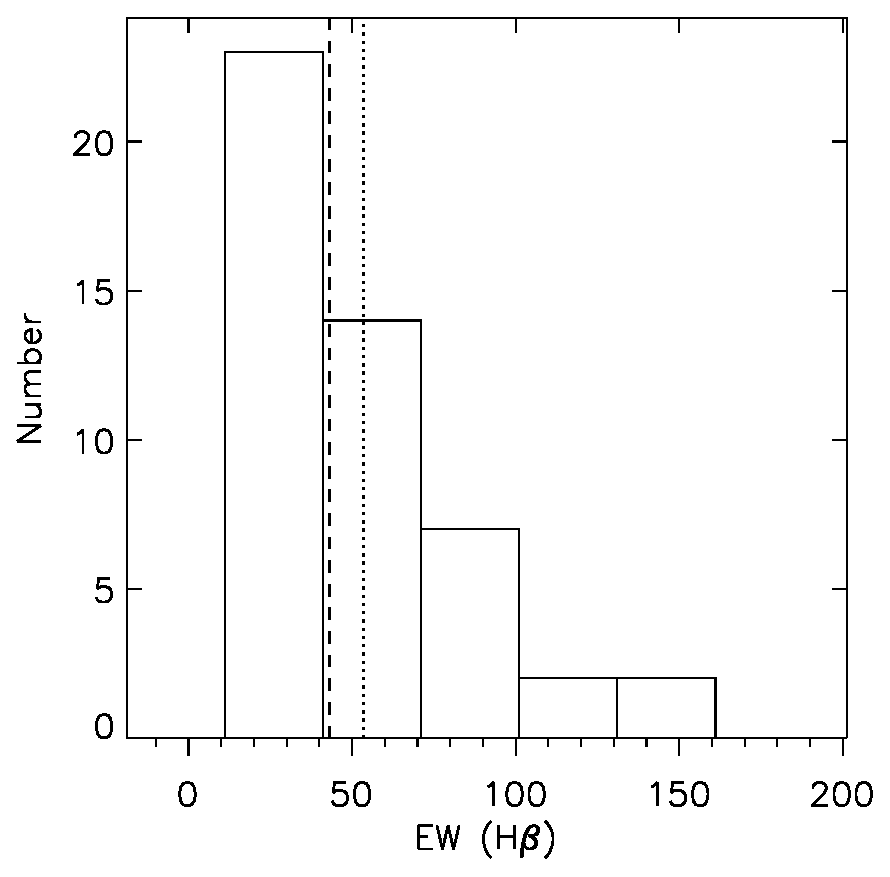
\includegraphics[width=12.0cm, height=8cm]{fig1.EPS}
\end{center}
\begin{center}
{. 1.     $\Lambda^{+} (\mu)$.
 $1,2,3$      $\alpha=3,0,-1$.}
\end{center}
\begin{center}
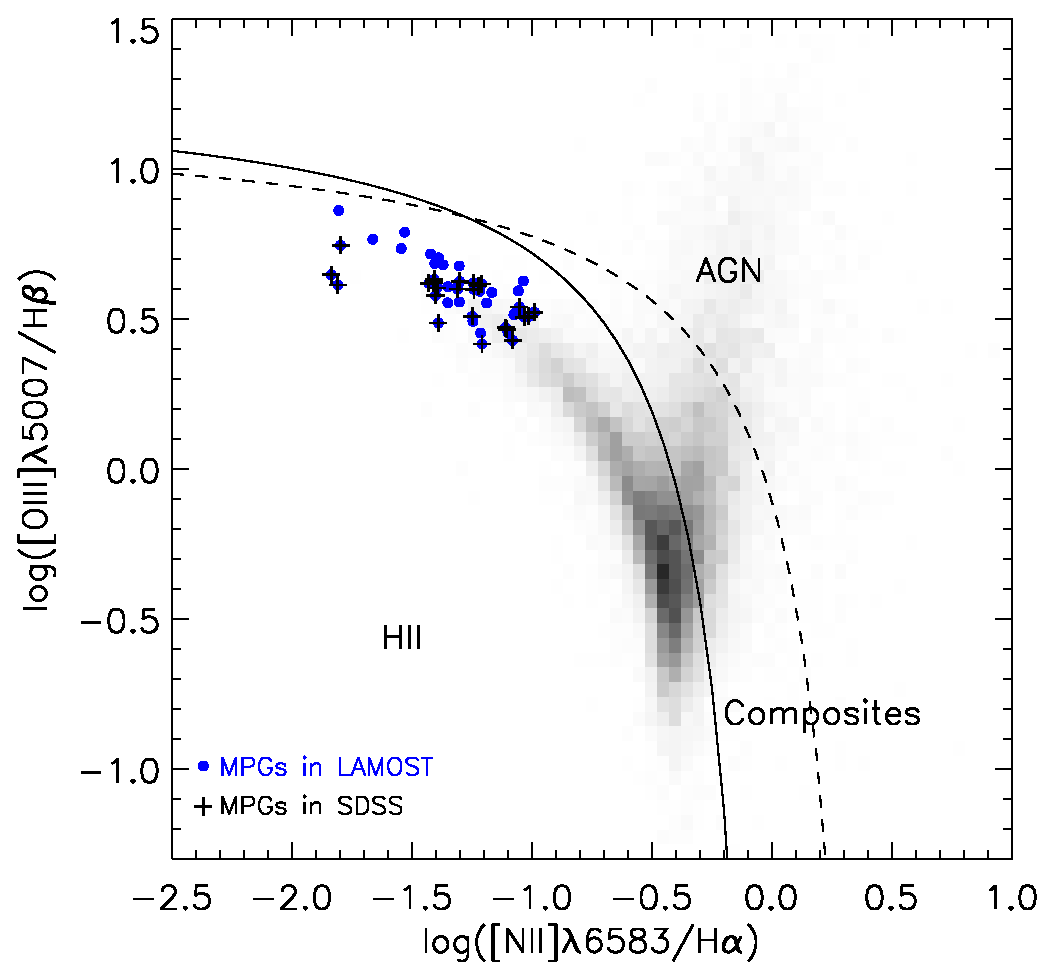
\includegraphics[width=12.0cm, height=8cm]{fig2.EPS}
\end{center}
\begin{center}
{. 2.     $\Lambda^{+}(\mu)$.
 $1,2,3$      $\alpha=3,0,-1$.}
\end{center}
\end{figure}

\clearpage


 :
$
\Omega=\omega/\omega_p.
$
, 
$$
\Omega\geqslant 0,\quad w_0=1-i\dfrac{\omega}{\nu}=1-i \dfrac{\Omega}{\varepsilon}=
-\dfrac{i(\Omega+i\varepsilon)}{\varepsilon}.
$$

     .

        :
$$
\Lambda(z)=\Lambda_{\infty}+\frac{\Lambda_2}{z^2}+
\frac{\Lambda_4}{z^4}+ \cdot \cdot \cdot , \ \quad z\to\infty.
\eqno {(3.3)}
$$
 (3.3)  :
$$
\Lambda_2=\frac{s_4(\alpha)-\eta^2_1s_2(\alpha)}{w_0\eta^2_1s_0(\alpha)}, \ \qquad
\Lambda_4=\frac{s_6(\alpha)-\eta^2_1s_4(\alpha)}{w_0\eta^2_1s_0(\alpha)},
\cdots.
$$
$$
s_n(\alpha)=\frac{1}{2}\int_{-\infty}^{\infty}\mu^n f_0(\mu,\alpha)d\mu=
\int_{0}^{\infty}\mu^n f_0(\mu, \alpha)d\mu.
$$

  (3.3) ,       
  $\pm\eta_0$   $\Lambda(z)$:
$$
\pm\eta_0\approx\sqrt{-\frac{\Lambda_2}{\Lambda_{\infty}}}.
\eqno {(3.4)}
$$
         .
  $\eta_0$       (3.4), 
$
\mathrm{Re}({w_0}/{\eta_0})>0.
$
    $\mathrm{exp}[-({w_0}/{\eta_0})x]$ 
   $x\to+\infty$.

 $\eta_0$   

$$
H_{\eta_{0}}(x,\mu)=\mathrm{exp}\left(-\frac{w_0}{\eta_0}x\right)\Phi(\eta_0,\mu),
$$
$$
e_{\eta_0}(x)=\mathrm{exp}\left(-\frac{w_0}{\eta_0}x\right)E_0.
$$

$$
\Phi(\eta_0,\mu)=\frac{E_0}{w_0}\frac{\eta_0\mu-\eta^2_1}{\eta_0-\mu}.
$$

      ( -  ). 
       \cite{Ashkroft}.

 (3.4)    :
$$
\eta_0=\eta_0(\alpha,\Omega,\varepsilon)\approx\sqrt{\frac{(\Omega+i\varepsilon)^2
[\eta^2_1s_2(\alpha)-s_4(\alpha)]}{w_0\eta^2_1s_0(\alpha)(\Omega^2-1+i\varepsilon \Omega)}}.
\eqno {(3.5)}
$$

 (3.5) ,    , ..  $\Omega\approx1$, .. 
$\omega\approx\omega_p$   $|\eta_0(\alpha,\Omega,\varepsilon)|$
        $\alpha$
  $\varepsilon\to 0$.

\begin{center}
  4.    
\end{center}


      ,  
  $\eta_0$  .  $\eta_0$  
    $\mu$, $\omega$  $\nu$,   
$(\alpha,\Omega,\varepsilon)$.
   $D^+(\alpha)$,  
  $(\Omega,\varepsilon)$, ,  
$(\Omega,\varepsilon)\in D^+(\alpha)$,    $N$  
$\Lambda(z)$  : $N=2$.  $D^-(\alpha)$    
 ,       : $N=0$.
,    ,   $L=L(\alpha)$.

    $(\Omega,\varepsilon)$ 
- $\mathbb R^2_+ = \{(\Omega,\varepsilon):\Omega\geqslant0,
\varepsilon\geqslant0\}$.  $\Omega\geqslant0$ ( $\omega=0$) 
   ,   $\varepsilon=0$ ( $\nu=0$)
   .

  $\mathrm\Gamma_{\rho}=C^+_{\rho}\cup C^-_{\rho}$,   
  $C^+_\rho$  $C^-_\rho$   $R=1/\rho$,
      ; $\rho$ - 
   , $C^{\pm}_\rho=\{z=x+iy, |z|=1/\rho,
|x\pm i\rho|\leqslant 1/\rho\}$.
 $R$   ,    
(  ),    $D_\rho$,  
$\mathrm\Gamma_\rho$. ,     $\rho\to0$   $D_\rho$
   $D_0$,
  $\mathrm\Gamma_0=\lim\limits_{\rho\to0}\mathrm\Gamma_\rho$.
          .

     \cite{Gahov}  $N$   
 $D_\rho$ :

$$
N=\frac{1}{2\pi i}\oint\limits_{\mathrm\Gamma_\rho}d\ln\Lambda(z).
$$

       $\rho\to0$  ,  
      , , 

$$
N=\frac{1}{2\pi i}\int_{-\infty}^{\infty}d\ln\Lambda^+(\tau)-
\frac{1}{2\pi i}\int_{-\infty}^{\infty}d\ln\Lambda^-(\tau).
$$

      $\tau\to-\tau$.  
 , , 
$$
N=\frac{1}{2\pi i}\int_{-\infty}^{\infty}d\ln\frac{\Lambda^+(\tau)}
{\Lambda^-(\tau)}.
$$

     -   $(-\infty,0)$  $(0,+\infty)$.
      . , 
$$
N=\frac{1}{\pi i}\int_{0}^{\infty}d\ln\frac{\Lambda^+(\tau)}
{\Lambda^-(\tau)}=2\varkappa_{\mathbb R_+}(G).
\eqno {(4.1)}
$$
 $\varkappa_{\mathbb R_+}(G)$ -  
$
G(\tau)={\Lambda^+(\tau)}/{\Lambda^-(\tau)},
$
    .

 ,  (4.1) ,     
$\Lambda(z)$     $G(\tau)$,
    .

     $\mathrm\Gamma_\alpha=\mathrm\Gamma(\alpha)$,
$$
\mathrm\Gamma(\alpha):z=G(\tau), \ 0\leqslant\tau\leqslant+\infty,
$$
,  $G(0)=1$, $\lim\limits_{\tau\to+\infty}G(\tau)=1$. ,
 (4.1),   $N$     
$\mathrm\Gamma(\alpha)$   , ..
$$
N=2\varkappa(G), \qquad \varkappa(G)=\mathrm{ind}_{[0,+\infty]}G(\tau).
$$

   $G(\mu)$    .   
$G(\mu)$  :
$$
G(\mu)=\frac{\Omega^+(\mu}{\Omega^-(\mu)},
$$

$$
\Omega^\pm(\mu)=(w_0-1)\eta^2_1+(\eta^2_1-\mu^2)\lambda_0(\mu,\alpha)\pm
is(\mu,\alpha)(\eta^2_1-\mu^2),
$$
$$
s(\mu,\alpha)=\frac{\pi}{2s_0(\alpha)}\mu f_0(\mu,\alpha).
$$

, 
$$
w_0-1=-i\frac{\omega}{\nu}=-i\frac{\Omega}{\varepsilon}, \ \ \ \ \
\eta^2_1=\varepsilon r(\alpha)(\varepsilon-i\Omega),
$$
$$
(w_0-1)\eta^2_1=-\Omega^2r(\alpha)-i\varepsilon\Omega r(\alpha)=
-\Omega(\Omega+i\varepsilon)r(\alpha).
$$

       $\Omega^\pm(\mu)$. :
$$
\Omega^\pm(\mu)=-P^\pm(\mu)-iQ^\pm(\mu),
$$

$$
P^\pm(\mu)=(1+\gamma)^2r(\alpha)+\lambda_0(\mu,\alpha)
(\mu^2-\varepsilon^2r(\alpha))\mp\varepsilon(1+\gamma)r(\alpha)s(\mu,\alpha),
$$
$$
Q^\pm(\mu)=\varepsilon(1+\gamma)r(\alpha)(1+\lambda_0(\mu,\alpha))\pm
(\mu^2-\varepsilon^2r(\alpha))s(\mu,\alpha).
$$

  $G(\mu)$   :
$$
G(\mu)=\frac{P^+(\mu)+iQ^+(\mu)}{P^-(\mu)+iQ^-(\mu)}.
$$

        $G(\mu)$:
$$
G(\mu,\alpha)=\frac{P^+P^-+Q^+Q^-}{(P^-)^2+(Q^-)^2}+i\frac{P^-Q^+-P^+Q^-}{(P^-)^2+(Q^-)^2},
$$
, ,
$$
G(\mu)=G_1(\mu)+iG_2(\mu),
$$

$$
G_1(\mu)=\frac{g_1(\mu)}{g(\mu)}, \qquad
G_2(\mu)=\frac{g_2(\mu)}{g(\mu)}.
$$


$$
g(\mu)=[P^-(\mu)]^2+[Q^-(\mu)]^2=$$$$=
[\Omega^2r(\alpha)+\lambda_0(\mu,\alpha)(\mu^2-\varepsilon^2r(\alpha))+
\varepsilon\Omega r(\alpha)s(\mu,\alpha)]^2+
$$
$$
+[\varepsilon\Omega(1+\lambda_0(\mu,\alpha))-s(\mu,\alpha)
(\mu^2-\varepsilon^2r(\alpha))]^2,
$$ \medskip
$$
g_1(\mu)=P^+(\mu)P^-(\mu)+Q^+(\mu)Q^-(\mu)=$$$$=
[\Omega^2r(\alpha)+\lambda_0(\mu,\alpha)(\mu^2-\varepsilon^2r(\alpha))]^2+
$$
$$
\hspace{3cm}+\varepsilon^2\Omega^2r^2(\alpha)[(1+\lambda_0(\mu,\alpha))^2-s^2(\mu,\alpha)]-
$$$$-
(\mu^2-\varepsilon^2r(\alpha))^2s^2(\mu,\alpha),
$$ \medskip
$$
g_2(\mu)=P^-(\mu)Q^+(\mu)-P^+(\mu)Q^-(\mu)=$$$$=
2s(\mu,\alpha)\big\{[\Omega2r(\alpha)+\lambda_0(\mu,\alpha)
(\mu^2-\varepsilon^2r(\alpha))]\times$$
$$\times(\mu^2-\varepsilon^2r(\alpha))+
\varepsilon^2\Omega^2r^2(\alpha)(1+\lambda_0(\mu,\alpha))\big\}.
$$

 (. . 3,4)    $(\Omega,\varepsilon)$
   $L_{\alpha}=L(\alpha,\Omega,\varepsilon)$,
    :
$$
L_\alpha=L_\alpha(\Omega,\varepsilon): \quad  g_1(\mu,\alpha,\Omega,\varepsilon)=0, \quad
g_2(\mu,\alpha,\Omega,\varepsilon)=0, \quad 0\leqslant\mu\leqslant+\infty,
$$
,         $G(\mu)$ 
   .

  $L_\alpha$    $(\Omega,\varepsilon)$ 
  $D^+(\alpha)$  $D^-(\alpha)$, ,    
$(\Omega,\varepsilon)$        $G(\mu)$
    .

     \cite{Lat1998TMF}  ,  
$(\Omega,\varepsilon)\in D^+(\alpha)$,
 $\varkappa_{[0,+\infty]}(G)=1$,   $(\Omega,\varepsilon)\in D^-(\alpha)$,
 $\varkappa_{[0,+\infty]}(G)=0$.    (  ) 
 $\mathrm\Gamma_\alpha$,  ,     .
   (  )      .

  (4.1) ,       
($N=2$),  $(\Omega,\varepsilon)\in D^+(\alpha)$,    
 ,  $(\Omega,\varepsilon)\in D^-(\alpha)$.

,    \cite{Lat1998TMF}     ,
 $(\Omega,\varepsilon)\in L_\alpha$.

     $L_\alpha$,  -
 $(\Omega,\varepsilon)$    $D^+(\alpha)$  $D^-(\alpha)$.

  $g_2(\mu,\alpha,\Omega,\varepsilon)=0$ :
$$
\Omega^2=-\frac{1}{r(\alpha)} \cdot
\frac{(\mu^2-\varepsilon^2r(\alpha))\lambda_0(\mu,\alpha)}{\mu^2+
\varepsilon^2r(\alpha)\lambda_0(\mu,\alpha)}.
\eqno {(4.2)}
$$

  $g_1(\mu,\alpha,\Omega,\varepsilon)=0$.   
   (4.2).      .  
$
g_1=P^-Q^+-P^+Q^-=0
$
,  $P^-=P^+({Q^-}/{Q^+})$.  , 
$$
 g_1\Big|_{g_2=0}=[P^-Q^+-P^+Q^-]\Bigg|_{P^-=\frac{Q^-}{Q^+}P^+}=
\frac{Q^-}{Q^+}\left[(P^+)^2+(P^-)^2\right].
$$

,   $g_1\big|_{g_2=0}=0$  
$Q^-(\mu)=0$.    , 
$$
\Omega\varepsilon r(\alpha)[1+\lambda_0(\mu,\alpha)]=
(\mu^2-\varepsilon^2r(\alpha))s(\mu,\alpha).
$$
      .    
$\Omega^2$   (4.2).    , 
$$
-\varepsilon^2r(\alpha)[1+\lambda_0(\mu,\alpha)]^2\frac{\lambda_0(\mu,\alpha)}
{\mu^2+\varepsilon^2r(\alpha)\lambda_0(\mu,\alpha)}=$$$$=s^2(\mu,\alpha)
(\mu^2-\varepsilon^2r(\alpha)),
$$
   :
$$
\varepsilon^2=-\frac{1}{r(\alpha)} \cdot \frac{\mu^2s^2(\mu,\alpha)}
{\lambda_0(\mu,\alpha)[(1+\lambda_0(\mu,\alpha))^2+s^2(\mu,\alpha)]}.
\eqno {(4.3)}
$$

    $\varepsilon^2$,  
(4.3),  (4.2).     :
$$
\Omega^2=-\frac{1}{r(\alpha)} \cdot
\frac{\mu^2[\lambda_0(\mu,\alpha)(1+\lambda_0(\mu,\alpha))+
s^2(\mu,\alpha)]^2}{\lambda_0(\mu,\alpha)[(1+\lambda_0(\mu,\alpha))^2+s^2(\mu,\alpha)]}.
\eqno {(4.4)}
$$

,       $L_\alpha$.
  (4.3)  (4.4)   :
$$
L_\alpha: \quad \Omega=\sqrt{L_1(\mu)}, \quad
\varepsilon=\sqrt{L_2(\mu)},\quad 0\leqslant\mu\leqslant+\infty.
\eqno {(4.5)}
$$

 (4.5)  :
$$
L_1(\mu)=\frac{s_0(\alpha)}{s_2(\alpha)} \cdot
\frac{\mu^2[\lambda_0(\mu,\alpha)(1+\lambda_0(\mu,\alpha))+s^2(\mu,\alpha)]^2}
{[-\lambda_0(\mu,\alpha)][(1+\lambda_0(\mu,\alpha))^2+s^2(\mu,\alpha)]}
$$

$$
L_2(\mu)=\frac{s_0(\alpha)}{s_2(\alpha)} \cdot \frac{\mu^2s_2(\mu,\alpha)}
{[-\lambda_0(\mu,\alpha)][(1+\lambda_0(\mu,\alpha))^2+s^2(\mu,\alpha)]}.
$$

,    $L_\alpha$,    $D^+(\alpha)$ 
$D^-(\alpha)$.
,   $(\Omega,\varepsilon)\in D^+(\alpha)$, 
$$
\varkappa(G)=\mathrm{ind}_{[0,+\infty]}\frac{\Lambda^+(\mu)}{\Lambda^-(\mu)}=1.
$$
 ,   $\mathrm\Gamma_\alpha$     .
  $(\Omega,\varepsilon)\in D^-(\alpha)$, 
$$
\varkappa(G)=\mathrm{ind}_{[0,+\infty]}\frac{\Lambda^+(\mu)}{\Lambda^-(\mu)}=0.
$$

 ,   $\mathrm\Gamma_\alpha$    .
 $\mathrm\Gamma(\alpha)$    $\mathbb C$  :
$$
\mathrm\Gamma_\alpha: \quad x=\mathrm{Re}\frac{\Lambda^+(\mu)}
{\Lambda^-(\mu)}, \quad y=\mathrm{Im}\frac{\Lambda^+(\mu)}
{\Lambda^-(\mu)}, \quad 0\leqslant\mu\leqslant+\infty.
$$


\begin{figure}
\begin{center}
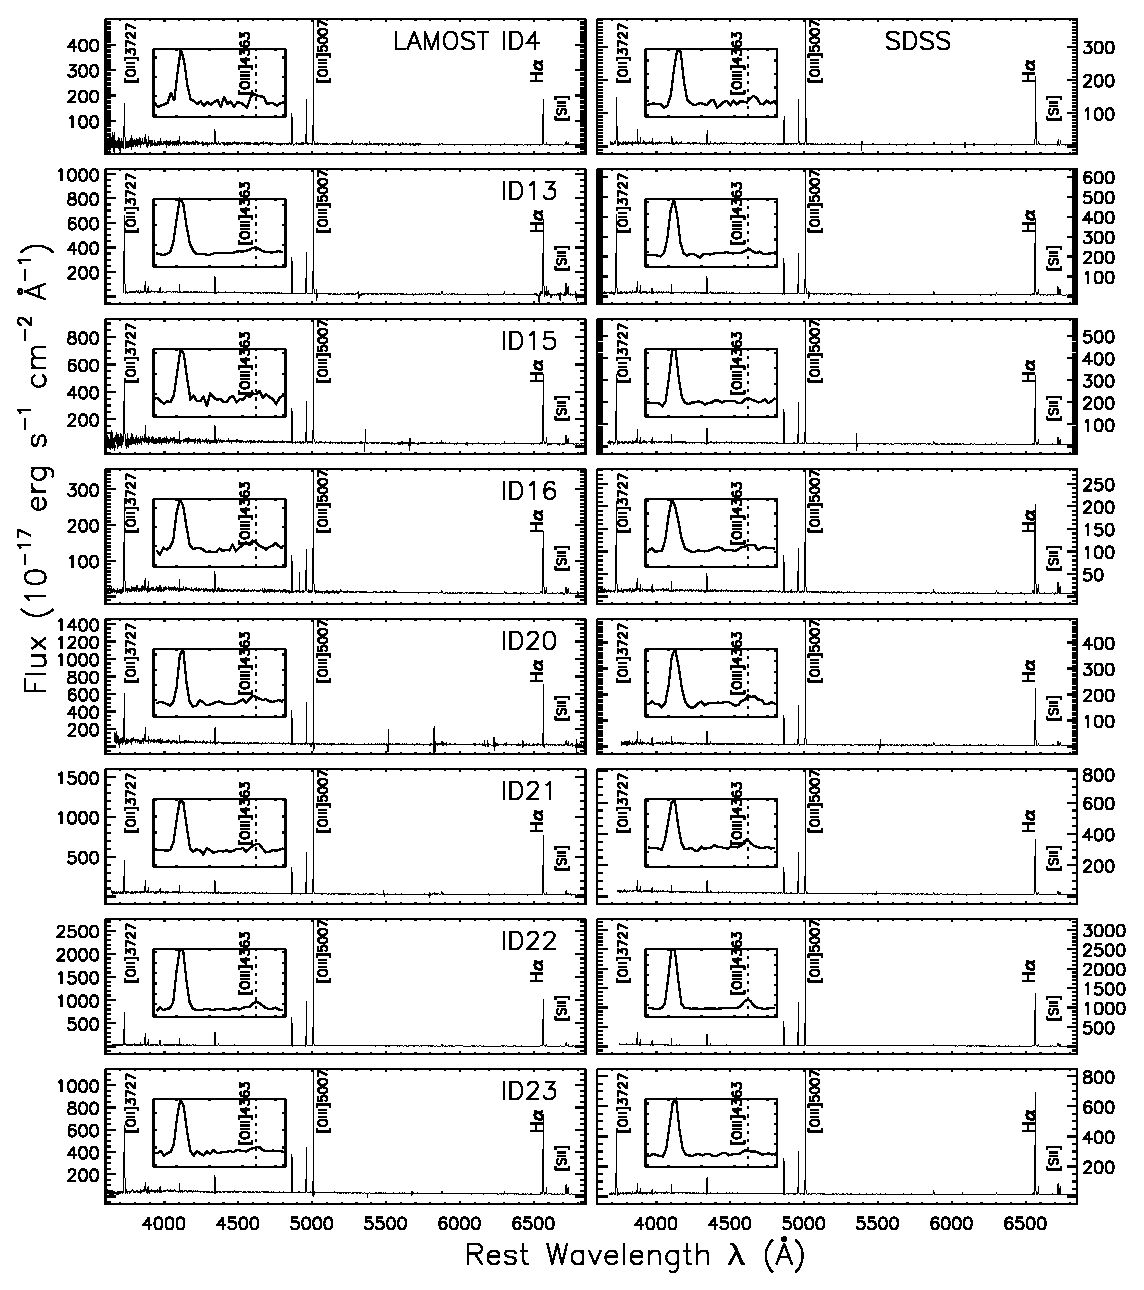
\includegraphics[width=13.0cm, height=10cm]{fig3.EPS}
\end{center}
\begin{center}
{. 3.  $L$   $D^+$  $D^-$.  $\alpha=-3$.}
\end{center}
\begin{center}
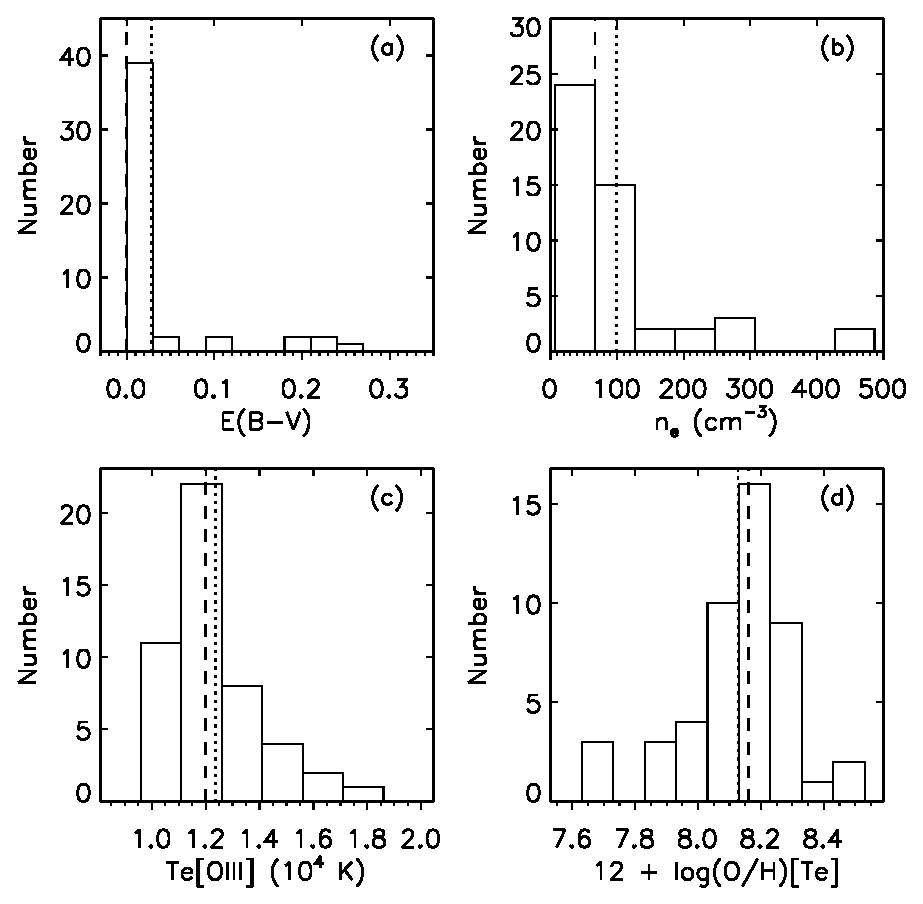
\includegraphics[width=13.0cm, height=10cm]{fig4.EPS}
\end{center}
\begin{center}
{. 4.  $L$   $D^+$  $D^-$.  $\alpha=3$.}
\end{center}
\end{figure}

\clearpage

,   $L_\alpha$    $(\Omega,\varepsilon)$
  :
$$
L(\alpha): \quad \mathrm{Re}\frac{\Lambda^+(\mu,\alpha,\Omega,\varepsilon)}
{\Lambda^-(\mu,\alpha,\Omega,\varepsilon)}=0, \quad
\mathrm{Im}\frac{\Lambda^+(\mu,\alpha,\Omega,\varepsilon)}
{\Lambda^-(\mu,\alpha,\Omega,\varepsilon)}=0, \quad 0\leqslant\mu\leqslant+\infty.
$$


    $\alpha$    
  : $-\infty\leqslant\alpha\leqslant+\infty$.
   $\alpha$=$-\infty$   ,  
$\alpha$=$+\infty$    .

     (,  ) :
  $H_{\eta_0}(x_1,\mu), e_{\eta_0}(x_1)$  (%$\equiv$
     $\Lambda(z)$  ,   
$G(\mu)=\Lambda^+(\mu)/\Lambda^-(\mu)$     ), 
$(\Omega,\varepsilon)\in D^+(\alpha)$,     ( 
    ,      
 ),  $(\Omega,\varepsilon)\in D^-(\alpha)$.


\begin{center}
  5.      
\end{center}


  ,   
(1.8)  (1.9)    (1.10)--(1.13).      
$$
H(x,\mu)=\dfrac{E_\infty}{w_0}\mu+\dfrac{E_0}{w_0}
\dfrac{\eta_0\mu-\eta_1^2}{\eta_0-\mu}
\exp\Big(-\dfrac{w_0x}{\eta_0}\Big)+$$$$+
\dfrac{1}{w_0}\int_{0}^{\infty}\exp\Big(-\dfrac{w_0x}{\eta}\Big)
F(\eta,\mu)\,E(\eta)\,d\eta,
\eqno{(5.1)}
$$
$$
e(x)=E_\infty+E_0\exp\Big(-\dfrac{w_0x}{\eta_0}\Big)+
\int_{0}^{\infty}\exp\Big(\dfrac{w_0x}{\eta}\Big)E(\eta)\,d\eta.
\eqno{(5.2)}
$$

   (5.1)  (5.2)  
  $E_0,\; E_\infty$     $E(\eta)$,
 $E_0=0$,  $(\Omega,\varepsilon)\in D^-(\alpha)$.

   $F(\eta,\mu)$   (5.1),    :
$$
H(x,\mu)=\dfrac{E_\infty}{w_0}\mu+\dfrac{E_0}{w_0}
\dfrac{\eta_0\mu-\eta_1^2}{\eta_0-\mu}
\exp\Big(-\dfrac{w_0x}{\eta_0}\Big)-
$$
$$
-\dfrac{1}{w_0}\int_{0}^{\infty}\exp\Big(-\dfrac{w_0x}{\eta}\Big)
\eta\,E(\eta)\,d\eta+$$$$+\dfrac{1}{w_0}\int_{0}^{\infty}
\exp\Big(-\dfrac{w_0x}{\eta}\Big)\dfrac{\eta^2-\eta_1^2}{\eta-\mu}
E(\eta)\,d\eta-
$$
$$
-\eta_1^2\exp\Big(-\dfrac{w_0x}{\mu}\Big)
\dfrac{\Lambda(\mu)}{\mu k(\mu,\alpha)}E(\mu)H(\mu), \quad -\infty<\mu<+\infty,\;x\geqslant 0.
\eqno{(5.3)}
$$

  (5.3)  (5.2)   
.    :
$$
w_0A=E_\infty\mu+E_0\dfrac{\eta_0\mu-\eta_1^2}{\eta_0-\mu}-
\int_{0}^{\infty}\eta E(\eta)\,d\eta+
$$
$$
+\int_{0}^{\infty}\dfrac{\eta^2-\eta_1^2}{\eta-\mu}E(\eta)\,d\eta-
w_0\eta_1^2\dfrac{\Lambda(\mu,\alpha)}{\mu k(\mu,\alpha)}E(\mu)H(\mu), \quad
0<\mu<+\infty,
\eqno{(5.4)}
$$
$$
E_\infty+E_0+\int_{0}^{\infty}E(\eta)\,d\eta=1.
\eqno{(5.5)}
$$

   (1.13).
       . :
$$
\int_{-\infty}^{+\infty}\mu F(\eta,\mu)f_0(\mu,\alpha)\,d\mu=$$$$=
-\int_{-\infty}^{+\infty}
\dfrac{\mu(\mu\eta-\eta_1^2)}{\mu-\eta}f_0(\mu,\alpha)\,d\mu-
2\eta_1^2w_0s_0(\alpha)\Lambda(\eta)=
$$
$$
=2\eta_1^2s_0(\alpha)-2w_0\eta_1^2s_0(\alpha)[1-\Lambda(\eta,\alpha)]-
2\eta_1^2w_0s_0(\alpha)\Lambda(\eta)=
$$
$$
=2\eta_1^2s_0(\alpha)(1-w_0)=i2\eta_1^2s_0(\alpha)\dfrac{\Omega}{\varepsilon}.
\eqno{(5.6)}
$$\bigskip
    
$F(\eta_0,\mu)$    :
$$
\int_{-\infty}^{\infty}\mu F(\eta_0,\mu)f_0(\mu,\alpha)\,d\mu=-\dfrac{1}{w_0}
\int_{-\infty}^{\infty}\mu\dfrac{\eta_0\mu-\eta_1^2}{\eta_0-\mu}f_0(\mu,\alpha)d\mu=
$$
$$
=2\eta_1^2(1-w_0)s_0(\alpha)=i2\eta_1^2s_0(\alpha)\dfrac{\Omega}{\varepsilon}.
\eqno{(5.7)}
$$
,     (5.6)  (5.7) .

        
$$
\int_{-\infty}^\infty \mu f_0(\mu,\alpha)\Bigg[E_\infty \mu+E_0\dfrac{\eta_0\mu-\eta_1^2}
{\eta_0-\mu}+\int_0^\infty F(\eta,\mu)E(\eta)d\eta\Bigg]d\mu=0,
$$
,       , , 
$$
E_\infty\int_{-\infty}^\infty \mu^2f_0(\mu,\alpha)d\mu+E_0\int_{-\infty}^\infty
\dfrac{\eta_0\mu-\eta_1^2}{\eta_0-\mu}\mu f_0(\mu,\alpha)d\mu+
$$
$$
+\int_0^\infty E(\eta)d\eta\int_{-\infty}^\infty \mu f_0(\mu,\alpha)F(\eta,\mu)d\mu=0.
\eqno{(5.8)}
$$
   (5.8) :
$$
\int_{-\infty}^\infty\mu^2f_0(\mu,\alpha)d\mu=2s_2(\alpha).
$$
   (5.8)    
$$
\Lambda(\eta_0)\equiv 1+\dfrac{\eta_0}{w_0\eta_1^2}\int_{-\infty}^\infty
\dfrac{\eta_1^2-\mu\eta_0}{\mu-\eta_0}k(\mu,\alpha)d\mu=0.
$$
    , 
$$
\int_{-\infty}^\infty\dfrac{\eta_0\mu-\eta_1^2}{\eta_0-\mu}\mu k(\mu,\alpha)d\mu=
\eta_1^2+\eta_0\int_{-\infty}^\infty\dfrac{\eta_1^2-\eta_0\mu}{\mu-\eta_0}k(\mu,\alpha)d\mu=
$$
$$
=\eta_1^2-w_0\eta_1^2=\eta_1^2(1-w_0)=\eta_1^2i\dfrac{\Omega}{\varepsilon}.
$$
 ,    :
$$
\int_{-\infty}^\infty\dfrac{\eta_0\mu-\eta_1^2}{\eta_0-\mu}\mu f_0(\mu,\alpha)d\mu=
2s_0(\alpha)\eta_1^2i\dfrac{\Omega}{\varepsilon}.
$$
      (5.8)    (5.6). 
   (5.8)    :
$$
2s_2(\alpha)E_\infty+E_02s_0(\alpha)\eta_1^2i\dfrac{\Omega}{\varepsilon}+
2s_0(\alpha)\eta_1^2i\dfrac{\Omega}{\varepsilon}\int_0^\infty E(\eta)d\eta=0,
$$

$$
r(\alpha)E_\infty+i\eta_1^2\dfrac{\Omega}{\varepsilon}
\Big(E_0+\int_0^\infty E(\eta)d\eta\Big)=0.
\eqno{(5.9)}
$$


   (5.5)  (5.9)     :
$$
r(\alpha)E_\infty+i\eta_1^2\dfrac{\Omega}{\varepsilon}(1-E_\infty)=0.
$$
     :
$$
E_\infty=-\dfrac{i\eta_1^2(\Omega/\varepsilon)}{r(\alpha)-i\eta_1^2(\Omega/\varepsilon)}=
$$$$=
-\dfrac{i\Omega(\varepsilon-i\Omega)}{1-i\Omega(\varepsilon-i\Omega)}=-
\dfrac{\Omega(\Omega+i\varepsilon)}{1-\Omega(\Omega+i\varepsilon)}.
\eqno{(5.10)}
$$

       (5.10).

 ,        
   $\eta=\eta_1$  $\eta=\infty$:
$$
E_\infty=\dfrac{\Lambda(\eta_1)}{\Lambda(\infty)}=\dfrac{\Lambda_1}{\Lambda_\infty}.
$$
  ,   , , 
$$
\dfrac{\Lambda_1}{\Lambda_\infty}=
\dfrac{1-{w_0}^{-1}}{1-{w_0}^{-1}+(w_0\varepsilon)^{-2}}=
-\dfrac{\Omega(\Omega+i\varepsilon)}{1-\Omega(\Omega+i\varepsilon)}.
$$

 (5.10) ,         , ..
      .

  (5.5)  (5.10) :
$$
E_0+\int_{0}^{\infty} E(\eta)\,d\eta=1-E_\infty=1-\dfrac{\Lambda_1}{\Lambda_\infty}=
$$
$$
=\dfrac{1}{1+w_0\varepsilon^2(w_0-1)}=\dfrac{1}{w_0\varepsilon^2\Lambda_\infty}=
\dfrac{\Lambda_1}{\Lambda_\infty w_0\varepsilon^2(w_0-1)}.
\eqno{(5.11)}
$$


     (5.4)  (5.11).  (5.4) 
     ,   (5.11) -- 
.

  
$$
N(z)=\int_{0}^{\infty}\dfrac{\eta^2-\eta_1^2}{\eta-z}E(\eta)\,d\eta,
\eqno{(5.12)}
$$
        :
$$
N^+(\mu)-N^-(\mu)=2\pi i (\mu^2-\eta_1^2)E(\mu),\quad 0<\mu<\infty.
\eqno{(5.13)}
$$

  (5.4)     
 
$$
\Lambda^+(\mu)[N^+(\mu)+\varphi(\mu)]=
\Lambda^-(\mu)[N^-(\mu)+\varphi(\mu)],\quad 0<\mu<+\infty.
\eqno{(5.14)}
$$

$$
\varphi(\mu)=-w_0A+E_\infty\mu+E_0\dfrac{\eta_0\mu-\eta_1^2}
{\eta_0-\mu}-\int_{0}^{\infty}\eta E(\eta)\,d\eta.
\eqno{(5.15)}
$$

     (5.14)   
  .
      
:    $X(z)$,   
 ,     $[0,+\infty]$,
     ,  
 $G(\mu)$   $[0,1]$,  ,   
 $X^{\pm}(\mu)$       $(0,+\infty)$
   :
$$
X^+(\mu)=G(\mu)X^-(\mu), \qquad 0<\mu<+\infty,
\eqno{(5.16)}
$$
, ,
$$
G(\mu)=\dfrac{\Lambda^+(\mu)}{\Lambda^-(\mu)}.
$$

  (5.16)     
       (  
):
$$
\ln X^+(\mu)-\ln X^-(\mu)=$$$$=\ln G(\mu)+2\pi k i, \quad
0<\mu<+\infty,\quad k=0,\pm 1,\pm 2, \cdots.
\eqno{(5.17)}
$$

  $\varkappa(G)=1$  $k=-1$,   
$\varkappa(G)=0$  $k=0$.      
     ,
   :
$$
\ln G(+\infty)-2\pi i \varkappa(G)=0.
$$

    (5.17)    
$$
\ln X(z)=\dfrac{1}{2\pi i}\int_{0}^{\infty}
\dfrac{\ln G(\tau)-2\pi i \varkappa(G)}{\tau-z}\,d\tau.
\eqno{(5.18)}
$$

      $V(z)$:
$$
V(z)=\dfrac{1}{2\pi i}\int_{0}^{\infty}
\dfrac{\ln G(\tau)-2\pi i \varkappa(G)}{\tau-z}\,d\tau.
$$


$$
X(z)=\exp V(z).
\eqno{(5.19)}
$$

,   (5.19)      
 $\varkappa(G)=1$.    
  (5.19)  :
$$
X(z)=\dfrac{1}{z}\exp\Big(\dfrac{1}{2\pi i}\int_{0}^{\infty}
\dfrac{\ln G(\tau,\alpha)-2\pi i}{\tau-z}\,d\tau\Big).
\eqno{(5.20)}
$$

,  $\varkappa(G)=0$   (5.16)  
(5.19),    $\varkappa(G)=1$ --  (5.20). 
    :
$$
X(z)=\dfrac{1}{z^\varkappa}\exp V(z),
$$
  $V(z)$   (5.18).


      
   (5.14)    
    ,   :
$$
X^+(\mu)[N^+(\mu)+\varphi(\mu)]=
X^-(\mu)[N^-(\mu)+\varphi(\mu)],\quad 0<\mu<+\infty.
\eqno{(5.21)}
$$

$$
X(z)=\dfrac{1}{z}\exp V(z),
$$

$$
V(z)=\dfrac{1}{\pi}\int_{0}^{\infty}\dfrac{\zeta(\tau)\,d\tau}
{\tau-z}, \qquad \zeta(\tau)=\dfrac{1}{2i}\ln G(\tau)-\pi.
$$

   $X(z)$   $\varphi(z)$,
  (5.15),    
(5.21):
$$
N(z)=w_0A-E_\infty z-E_0\dfrac{\eta_0 z-\eta_1^2}{\eta_0-z}+
\int_{0}^{\infty}\eta E(\eta)\,d\eta+$$$$
+\dfrac{1}{X(z)}\Big(C_0+\dfrac{C_{-1}}{z-\eta_0}\Big),
\eqno{(5.22)}
$$
 $C_0$  $C_1$ --  .

    (5.22)  $z\to \infty$:
$$
N(z)=w_0A-E_\infty z+E_0\eta_0+\int_{0}^{\infty}\eta
E(\eta)\,d\eta+C_0z+
$$
$$
+C_{-1}-C_0V_1+o(1),\quad z\to \infty.
\eqno{(5.23)}
$$
   (5.22)       
(5.23), 
$$
C_0=E_\infty.
\eqno{(5.24)}
$$

  $N(\infty)=0$   (5.24)   :
$$
w_0A=-E_0\eta_0-\int_{0}^{\infty}\eta
E(\eta)\,d\eta-C_{-1}+E_\infty V_1,
\eqno{(5.25)}
$$

$$
V_1=-\dfrac{1}{\pi}\int_{0}^{\infty}\zeta(\tau)d\tau.
$$
   (5.22)    $\eta_0$, :
$$
C_{-1}=-E_0(\eta_0^2-\eta_1^2)X(\eta_0).
\eqno{(5.26)}
$$

     $E_0$,   $A_+$ 
   $E(\eta)$.

   $E(\eta)$ ,   
 (5.22)    (5.13),     (5.12).
  :
$$
E(\eta)=\dfrac{1}{2\pi i(\eta^2-\eta_1^2)}\Big(C_0+
\dfrac{C_{-1}}{\eta-\eta_0}\Big)\Big(\dfrac{1}{X^+(\eta)}-
\dfrac{1}{X^-(\eta)}\Big).
\eqno{(5.27)}
$$


  $E_0$  (5.27)   (5.5). :
$$
E_\infty+E_0+\dfrac{1}{2\pi i}\int_{0}^{\infty}
\Big(\dfrac{1}{X^+(\eta)}-\dfrac{1}{X^-(\eta)}\Big)\Big(E_\infty-
$$$$-
\dfrac{E_0X(\eta_0)(\eta_0^2-\eta_1^2)}{\eta-\eta_0}\Big)\dfrac{d\eta}
{\eta^2-\eta_1^2}=1.
\eqno{(5.28)}
$$

   (5.28)     
    .
    :
$$
\dfrac{1}{X(z)}-z+V_1(\alpha)=$$$$=\dfrac{1}{2\pi i}\int_{0}^{\infty}
\Big(\dfrac{1}{X^+(\eta)}
-\dfrac{1}{X^-(\eta)}\Big)\dfrac{d\eta}{\eta-z},\quad
z\in \mathbb{C}\setminus [0,+\infty].
\eqno{(5.29)}
$$
:
$$
J_1=\dfrac{1}{2\pi i}\int_{0}^{\infty}
\Big(\dfrac{1}{X^+(\eta)}-\dfrac{1}{X^-(\eta)}\Big)\dfrac{d\eta}
{\eta^2-\eta_1^2}=\dfrac{1}{2\eta_1}\Big(J(\eta_1)-J(-\eta_1)\Big),
$$

$$
J(\pm\eta_1)=\dfrac{1}{2\pi i}\int_{0}^{\infty}
\Big(\dfrac{1}{X^+(\eta)}-\dfrac{1}{X^-(\eta)}\Big)\dfrac{d\eta}
{\eta \mp \eta_1}.
$$
 (5.29) :
$$
J(\pm \eta_1)=\dfrac{1}{X(\pm\eta_1)}\mp\eta_1+V_1.
$$
,     (5.28) :
$$
J_1=\dfrac{1}{2\eta_1}\Big[\dfrac{1}{X(\eta_1)}-\dfrac{1}{X(-\eta_1)}
-2\eta_1\Big]=$$$$=
-1-\dfrac{X(\eta_1)-X(-\eta_1)}{2\eta_1X(\eta_1)X(-\eta_1)}.
$$

    
$$
\Lambda(z)=\Lambda_\infty (\eta_0^2-z^2)X(z)X(-z), \qquad z\in
\mathbb{C}\setminus [-\infty,+\infty].
$$

    $z=\eta_1$, :
$$
\Lambda_1=\Lambda_\infty(\eta_0^2-\eta_1^2)X(\eta_1)X(-\eta_1),
$$

$$
X(\eta_1)X(-\eta_1)=\dfrac{E_\infty}{\eta_0^2-\eta_1^2}.
$$

,   
$$
\alpha^{\pm}=\dfrac{X(\eta_1)\pm X(-\eta_1)}{2},
$$

$$
J_1=-1-\dfrac{\alpha^-(\eta_0^2-\eta_1^2)}{\eta_1 E_\infty}.
$$

   (5.28)
$$
J_2=\dfrac{1}{2\pi i}\int_{0}^{\infty}
\Big(\dfrac{1}{X^+(\eta)}-\dfrac{1}{X^-(\eta)}\Big)\dfrac{d\eta}
{(\eta^2-\eta_1^2)(\eta-\eta_0)}
$$
      . , 
  .  ,   . 5.


\begin{figure}
\begin{center}
\includegraphics[width=13cm, height=13cm]{file5.EPS}
\end{center}
\begin{center}
{. 5.  .}
\end{center}
\end{figure}


  ,   , :
$$
J_2=\Big[\Res_{\eta_1}+\Res_{-\eta_1}+\Res_{\eta_0}\Big]
\dfrac{1}{X(z)(z^2-\eta_1^2)(z-\eta_0)}=
$$
$$
=\dfrac{1}{2\eta_1}\Big[\dfrac{1}{X(\eta_1)(\eta_1-\eta_0)}+
\dfrac{1}{X(-\eta_1)(\eta_1+\eta_0)}\Big]+
\dfrac{1}{X(\eta_0)(\eta_0^2-\eta_1^2)}.
$$

  (5.26)   :
$$
J_2=\dfrac{\eta_1[X(\eta_1)+X(-\eta_1)]-\eta_0[X(\eta_1)-X(-\eta_1)]}
{2\eta_1 X(\eta_1)X(-\eta_1)(\eta_1^2-\eta_0^2)}-\dfrac{E_0}{C_{-1}},
$$

$$
J_2=-\dfrac{\eta_1\alpha^+-\eta_0\alpha^-}{\eta_1E_\infty}+
\dfrac{1}{X(\eta_0)(\eta_0^2-\eta_1^2)}.
$$

   $J_1$  $J_2$  (5.28).  ,   :
$$
E_0=\dfrac{E_\infty(\eta_1/(\eta_0^2-\eta_1^2)+\alpha^-)}
{X(\eta_0)(\eta_1\alpha^+-\eta_0\alpha^-)}.
\eqno{(5.30)}
$$

  (5.30)  (5.26) , 
$$
C_{-1}=-\dfrac{E_\infty[\eta_1+\alpha^-(\eta_0^2-\eta_1^2)]}
{\eta_1\alpha^+-\eta_0\alpha^-}.
$$

    $A$.     
$$
\int_{0}^{\infty}\eta\,E(\eta)\,d\eta=C_0
\int_{0}^{\infty}\Big(\dfrac{1}{X^+(\eta)}-\dfrac{1}{X^-(\eta)}\Big)
\dfrac{\eta\,d\eta}{\eta^2-\eta_1^2}+$$
$$
+C_{-1}\dfrac{1}{2\pi i}\int_{0}^{\infty}
\Big(\dfrac{1}{X^+(\eta)}-\dfrac{1}{X^-(\eta)}\Big)
\dfrac{\eta\,d\eta}{(\eta^2-\eta_1^2)(\eta-\eta_0)}.
\eqno{(5.31)}
$$

        .
, 
$$
\int_{0}^{\infty}\Big(\dfrac{1}{X^+(\eta)}-\dfrac{1}{X^-(\eta)}\Big)
\dfrac{\eta\,d\eta}{\eta^2-\eta_1^2}=\dfrac{J(\eta_1)+J(-\eta_1)}{2}=
$$
$$
=\dfrac{1}{2}\Big[\dfrac{1}{X(\eta_1)}+\dfrac{1}{X(-\eta_1)}+
2\eta_1\Big]=V_1+\dfrac{\alpha^+}{X(\eta_1)X(-\eta_1)}=$$$$=
V_1+\dfrac{\alpha^+}{E_\infty}(\eta_0^2-\eta_1^2).
$$

      :
$$
\dfrac{1}{2\pi i}\int_{0}^{\infty}
\Big(\dfrac{1}{X^+(\eta)}-\dfrac{1}{X^-(\eta)}\Big)\dfrac{\eta\,d\eta}
{(\eta^2-\eta_1^2)(\eta-\eta_0)}=
$$
$$=
\Big[\Res_{\infty}+\Res_{\eta_1}+\Res_{-\eta_1}+\Res_{\eta_0}\Big]
\dfrac{z}{(z^2-\eta_1^2)(z-\eta_0)}=$$$$
=-1+\dfrac{1}{2X(\eta_1)(\eta_1-\eta_0)}-\dfrac{1}{X(-\eta_1)
(\eta_1+\eta_0)}+$$$$+\dfrac{\eta_0}{X(\eta_0)(\eta_0^2-\eta_1^2)}=
-1-\dfrac{\eta_0\alpha^+-\eta_1\alpha^-}{E_\infty}+
\dfrac{\eta_0}{X(\eta_0)(\eta_0^2-\eta_1^2)}.
$$

     (5.31). :
$$
\int_{0}^{\infty}\eta\,E(\eta)\,d\eta=
E_\infty V_1+\alpha^+(\eta_0^2-\eta_1^2)-$$$$
-C_{-1}-\dfrac{C_{-1}}{E_\infty}
(\eta_0\alpha^+-\eta_1\alpha^-)- \eta_0 E_0.
$$


     (5.25) , 
$$
w_0A=-\eta_1\dfrac{\eta_0\alpha^+-\eta_1\alpha^-+(\eta_0^2-\eta_1^2)
[(\alpha^+)^2-(\alpha^-)^2]}{\eta_1\alpha^+-\eta_0\alpha^-}.
$$

   $\alpha^{\pm}$    
,  , 
$$
(\alpha^+)^2-(\alpha^-)^2=X(\eta_1)X(-\eta_1)=\dfrac{E_\infty}
{\eta_0^2-\eta_1^2}.
$$
,    :
$$
w_0A=-\eta_1\dfrac{E_\infty+\eta_0\alpha^+-\eta_1\alpha^-}
{\eta_1\alpha^+-\eta_0\alpha^-}.
\eqno{(5.32)}
$$

       .   
 (5.1)  (5.2).      (5.10),
(5.27), (5.30)  (5.32).


\begin{center}
  
\end{center}


,          
,      ,   
 .         
   .
         
       .
      .  
          .
      .   
      (   
 ).       
        
.

,      $(\Omega, \varepsilon)$ 
 $D^(\alpha)$,   $L_\alpha$, ,  
$(\Omega, \varepsilon) \in D^+(\alpha)$  
,   $(\Omega, \varepsilon) \in D^-(\alpha)$  .

,         
       (., , \cite{Chizhonkov},
\cite{Morozov}).         
    (. \cite{Vedenyapin}).



\end{document}
